\documentclass[12pt]{article}
\usepackage{graphicx}
\usepackage{epstopdf}
  
%
% Title[Enter title of the experiment here]
\title{EE230: Experiment No.03\\
Opamps circuits\\}

% Author[Enter details of author here]
\author{Mudavath vishnuvardhan,200070044}

% begin the document.
\begin{document}

% make a title page.[this creates title page]
\maketitle

\section{Overview of the experiment} %[This segment creates Section as seen in document]

\subsection{Aim of the experiment}%[This segment creates sebsections under the same section]
Aim of this experiment is using Opamp to make half wave , full wave rectifier and improving them from that made using diodes (bridge rectifier).

\subsection{ Methods}

I used ngspice software to write code for half wave precision rectifier and improved half wave precision rectifier,full wave rectifier and performed transient analysis, plotted time vs \(v_{in}\), \(v_{out}\) for all three circuits for a sinusodial input 10pp  and then extracted output files from each .cir ngspice file in .txt format and then used matplotlib to visualise this data from text file .
\newpage

\section{Design}%[To add multiple sections, keep appending blocks like this]

\subsection{Half-wave Precision rectifier}

connect a 10v peak to peak sinusodial voltage as shown below and measure vout at load resistance (\(R_{l}\)).\\
for \(v_{in}=5sin(wt)\):\\
when \(v_{in}\) is positive both diodes get forward biased and resistance \(R_{2}\) gets shorted thus voltage across \(v_{out}\) goes to zero, when \(v_{in}\) is negative diodes gets reverse biaseda nd thus no current flows through diodes thus whole circuit behaves as inverting amplifier with gain unity thus we get \(v_{out} = -v_{in}\).  
 \begin{figure}[h!]
\centering
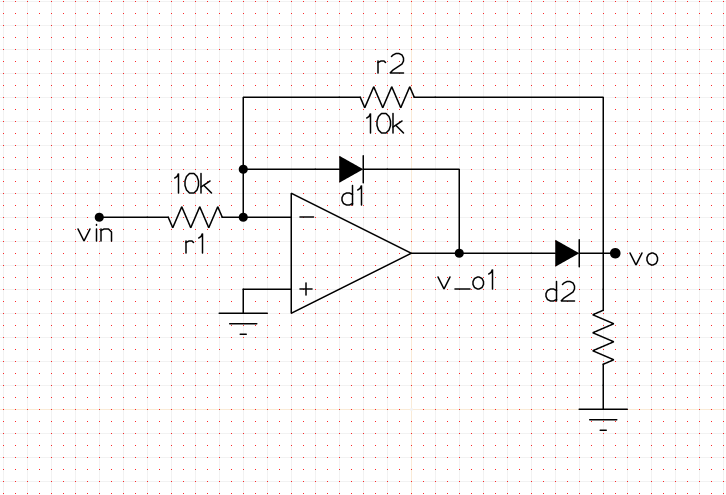
\includegraphics[scale = 0.6]{half_wave_rectifier.png}
\end{figure}
\newpage

 
\subsection{Improved Half-wave Precision rectifier}
connect a 10v peak to peak sinusodial voltage as shown below and measure vout at load resistance (\(R_{l}\)).\\
for \(v_{in}=5sin(wt)\):\\
when \(v_{in}\) is positive both diodes get reverse biased and thus no current flows through diodes thus whole circuit behaves as inverting amplifier with gain unity thus we get \(v_{out} = -v_{in}\)and when \(v_{in}\) is negative diodes gets forward biased ,resistance \(R_{2}\) gets shorted thus voltage across \(v_{out}\) goes to zero, 
\begin{figure}[h!]
\centering
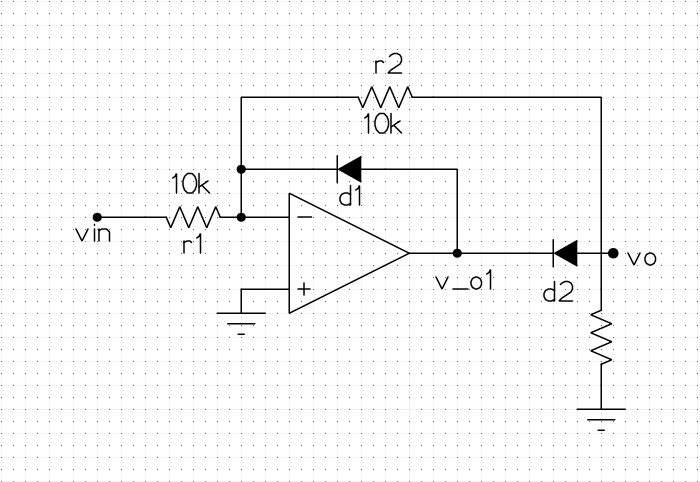
\includegraphics[scale = 0.6]{improved_half_wave_rectifier.png}
\end{figure}
\newpage

\subsection{Full-wave Precision rectifier}
connect a 10v peak to peak sinusodial voltage as shown below and measure vout at load resistance (\(R_{l}\)).\\
for \(v_{in}=5sin(wt)\):\\
when \(v_{in}\) is positive both diodes get reverse biased and thus no current flows through diodes thus Improved half wave rectifier part of the circuit behaves as inverting amplifier with gain unit thus we get \(v_{Improved-half-rectifier} = -v_{in}\) thus \(v_{out}=V_{in}\) and when \(v_{in}\) is negative diodes gets forward biased ,resistance \(R_{2}\) gets shorted thus voltage across \(v_{Improved-half-rectifier}\) goes to zero thus \(v_{out}=V_{in}\). 
\begin{figure}[h!]
\centering
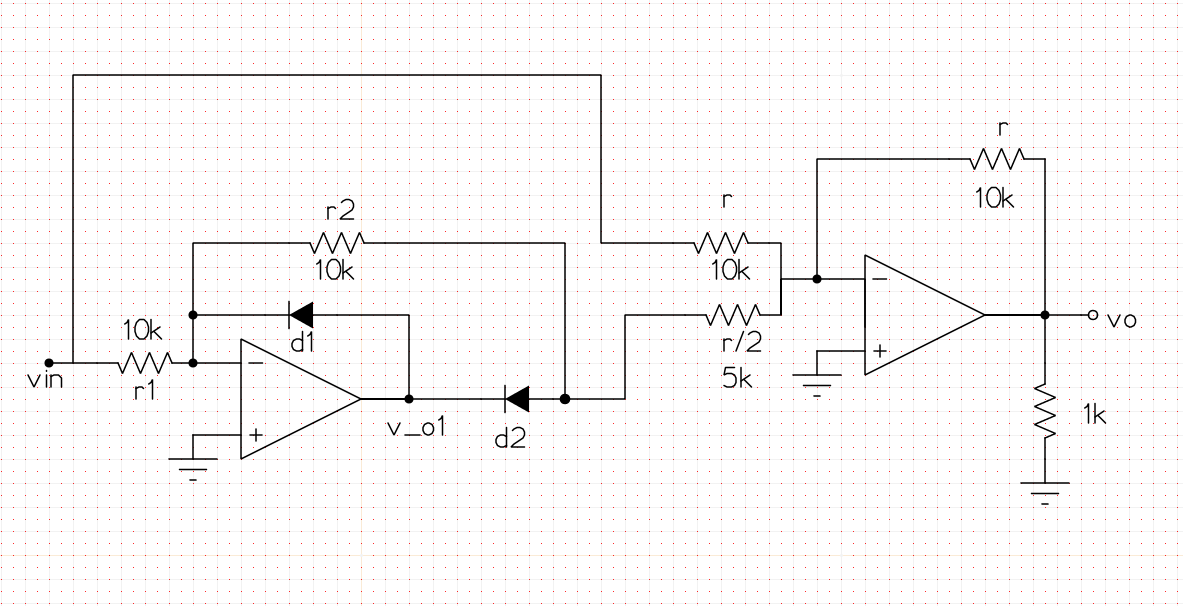
\includegraphics[scale = 0.4]{full_wave_rectifier.png}
\end{figure}
\newpage

 
\section{Simulation results}%[One more section]
\subsection{Code snippet}

\subsubsection{Half-wave rectifier}
Half wave precision rectifier\\
.subckt ua741    1  2  3  4  5\\
c1   11 12 8.661E-12\\
c2    6  7 30.00E-12\\
dc    5 53 dx\\
de   54  5 dx\\
dlp  90 91 dx\\
dln  92 90 dx\\
dp    4  3 dx\\
egnd 99  0 poly(2) (3,0) (4,0) 0 .5 .5\\
fb    7 99 poly(5) vb vc ve vlp vln 0 10.61E6 -10E6 10E6 10E6 -10E6\\
ga    6  0 11 12 188.5E-6\\
gcm   0  6 10 99 5.961E-9\\
iee  10  4 dc 15.16E-6\\
hlim 90  0 vlim 1K\\
q1   11  2 13 qx\\
q2   12  1 14 qx\\
r2    6  9 100.0E3\\
rc1   3 11 5.305E3\\
rc2   3 12 5.305E3\\
re1  13 10 1.836E3\\
re2  14 10 1.836E3\\
ree  10 99 13.19E6\\
ro1   8  5 50\\
\newpage
ro2   7 99 100\\
rp    3  4 18.16E3\\
vb    9  0 dc 0\\
vc    3 53 dc 1\\
ve   54  4 dc 1\\
vlim  7  8 dc 0\\
vlp  91  0 dc 40\\
vln   0 92 dc 40\\
.model dx D(Is=800.0E-18 Rs=1)\\
.model qx NPN(Is=800.0E-18 Bf=93.75)\\
.ends\\
.include Diode\_1N914.txt\\
x1 0 2  6 7 4 ua741\\
d2 2 4 1N914\\
d3 4 3 1N914\\
vin 1 0 sin(0 5 1k 0 0)\\
vcc1 6 0 15v\\
vcc2 7 0 -15v\\
r1 1 2 10k\\
r2 2 3 10k\\
rl 3 0 1k\\
.tran 1us 4ms\\  
.control\\
run\\
plot v(3) v(4) v(1)\\
print v(3) v(4) v(1)\\
.endc \\
.end\\
\newpage\\

\subsubsection{Improved half-wave rectifier}
Improved Half wave precision rectifier\\
.subckt ua741    1  2  3  4  5\\
c1   11 12 8.661E-12\\
c2    6  7 30.00E-12\\
dc    5 53 dx\\
de   54  5 dx\\
dlp  90 91 dx\\
dln  92 90 dx\\
dp    4  3 dx\\
egnd 99  0 poly(2) (3,0) (4,0) 0 .5 .5\\
fb    7 99 poly(5) vb vc ve vlp vln 0 10.61E6 -10E6 10E6 10E6 -10E6\\
ga    6  0 11 12 188.5E-6\\
gcm   0  6 10 99 5.961E-9\\
iee  10  4 dc 15.16E-6\\
hlim 90  0 vlim 1K\\
q1   11  2 13 qx\\
q2   12  1 14 qx\\
r2    6  9 100.0E3\\
rc1   3 11 5.305E3\\
rc2   3 12 5.305E3\\
re1  13 10 1.836E3\\
re2  14 10 1.836E3\\
ree  10 99 13.19E6\\
ro1   8  5 50\\
\newpage
ro2   7 99 100\\
rp    3  4 18.16E3\\
vb    9  0 dc 0\\
vc    3 53 dc 1\\
ve   54  4 dc 1\\
vlim  7  8 dc 0\\
vlp  91  0 dc 40\\
vln   0 92 dc 40\\
.model dx D(Is=800.0E-18 Rs=1)\\
.model qx NPN(Is=800.0E-18 Bf=93.75)\\
.ends\\
.include Diode\_1N914.txt\\
x1 0 2  6 7 4 ua741\\
d2 4 2 1N914\\
d3 3 4 1N914\\
vin 1 0 sin(0 5 1k 0 0)\\
vcc1 6 0 15v\\
vcc2 7 0 -15v\\
r1 1 2 10k\\
r2 2 3 10k\\
rl 3 0 1k\\
.tran 1us 4ms\\  
.control\\
run\\
plot v(3) v(4) v(1)\\
print v(3) v(4) v(1)\\
.endc \\
.end\\
\newpage

\subsubsection{full-wave rectifier}
full wave precision rectifier\\
.subckt imprect 1 3 \\
.subckt ua741    1  2  3  4  5\\
c1   11 12 8.661E-12\\
c2    6  7 30.00E-12\\
dc    5 53 dx\\
de   54  5 dx\\
dlp  90 91 dx\\
dln  92 90 dx\\
dp    4  3 dx\\
egnd 99  0 poly(2) (3,0) (4,0) 0 .5 .5\\
fb    7 99 poly(5) vb vc ve vlp vln 0 10.61E6 -10E6 10E6 10E6 -10E6\\
ga    6  0 11 12 188.5E-6\\
gcm   0  6 10 99 5.961E-9\\
iee  10  4 dc 15.16E-6\\
hlim 90  0 vlim 1K\\
q1   11  2 13 qx\\
q2   12  1 14 qx\\
r2    6  9 100.0E3\\
rc1   3 11 5.305E3\\
\newpage
rc2   3 12 5.305E3\\
re1  13 10 1.836E3\\
re2  14 10 1.836E3\\
ree  10 99 13.19E6\\
ro1   8  5 50\\
ro2   7 99 100\\
rp    3  4 18.16E3\\
vb    9  0 dc 0\\
vc    3 53 dc 1\\
ve   54  4 dc 1\\
vlim  7  8 dc 0\\
vlp  91  0 dc 40\\
vln   0 92 dc 40\\
.model dx D(Is=800.0E-18 Rs=1)\\
.model qx NPN(Is=800.0E-18 Bf=93.75)\\
.ends\\
.include Diode\_1N914.txt\\
x1 0 2  6 7 4 ua741\\
d2 4 2 1N914\\
d3 3 4 1N914\\
r1 1 2 10k\\
r2 2 3 10k\\
vcc1 6 0 15v\\
vcc2 7 0 -15v\\
.ends\\
\newpage
.subckt ua741    1  2  3  4  5\\
c1   11 12 8.661E-12\\
c2    6  7 30.00E-12\\
dc    5 53 dx\\
de   54  5 dx\\
dlp  90 91 dx\\
dln  92 90 dx\\
dp    4  3 dx\\
egnd 99  0 poly(2) (3,0) (4,0) 0 .5 .5\\
fb    7 99 poly(5) vb vc ve vlp vln 0 10.61E6 -10E6 10E6 10E6 -10E6\\
ga    6  0 11 12 188.5E-6\\
gcm   0  6 10 99 5.961E-9\\
iee  10  4 dc 15.16E-6\\
hlim 90  0 vlim 1K\\
q1   11  2 13 qx\\
q2   12  1 14 qx\\
r2    6  9 100.0E3\\
rc1   3 11 5.305E3\\
rc2   3 12 5.305E3\\
re1  13 10 1.836E3\\
re2  14 10 1.836E3\\
ree  10 99 13.19E6\\
\newpage
ro1   8  5 50\\
ro2   7 99 100\\
rp    3  4 18.16E3\\
vb    9  0 dc 0\\
vc    3 53 dc 1\\
ve   54  4 dc 1\\
vlim  7  8 dc 0\\
vlp  91  0 dc 40\\
vln   0 92 dc 40\\
.model dx D(Is=800.0E-18 Rs=1)\\
.model qx NPN(Is=800.0E-18 Bf=93.75)\\
.ends\\
xx1 1 2 imprect\\
xx2 0 3 6 7 4 ua741\\
vin 1 0 sin(0 5 1k 0 0)\\
vcc1 6 0 15\\
vcc2 7 0 -15\\
r1 1 3 10k\\
r2 2 3 5k\\
r3 3 4 10k\\
rl 4 0 1k\\
.tran 1us 4ms\\  
.control\\
run\\
plot v(4) v(1)\\
print v(4) v(1)\\
.endc \\
.end\\
\newpage


\subsection{Simulation results}
\subsubsection{half wave precision rectifier}
X-axis is time axis, Y-axis is voltage axis time vs \(V_{in}\), \(V_{out}\),\(V_{diode}\) is plotted below . plot shows that when \(V_{in}\) is sinusodial at \(V_{out}\) negative part of sinusodial curve is inverted and  positive part of vin is returned as 0v .\\
\begin{figure}[h!]
\centering
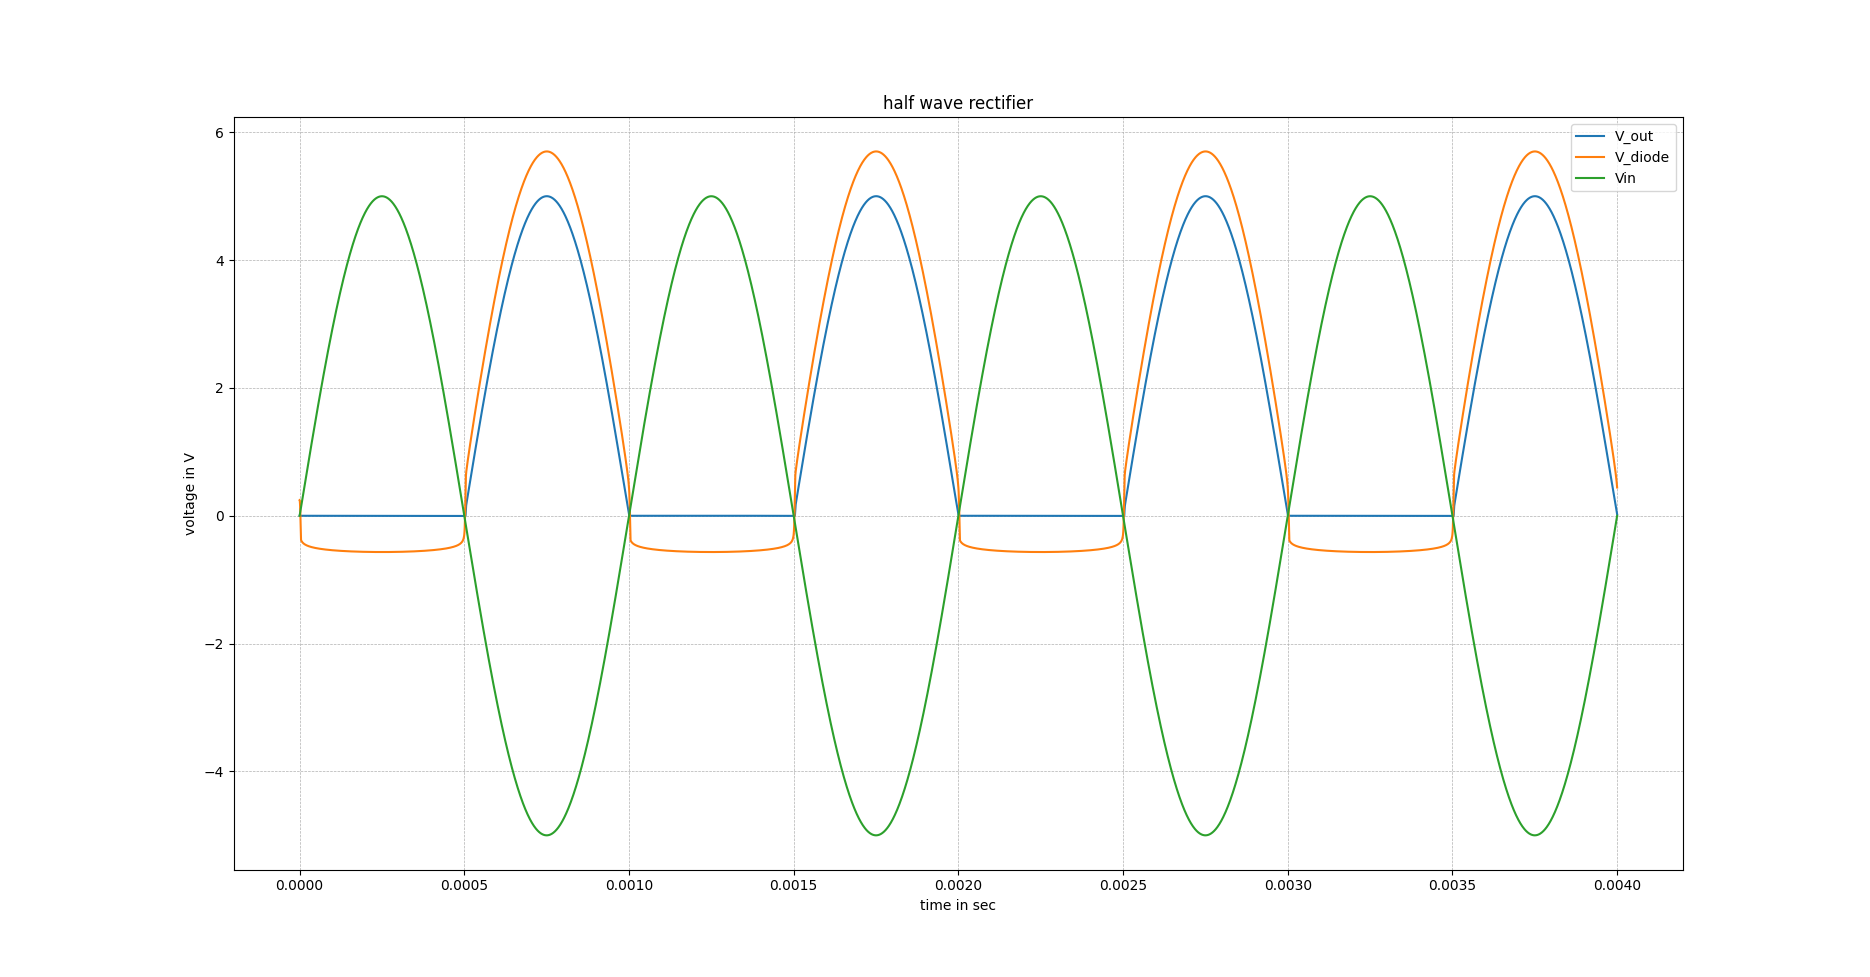
\includegraphics[scale = 0.4]{half_wave_rect_plot.png}
\end{figure}
\newpage


\subsubsection{improved half wave rectifier}
X-axis is time axis, Y-axis is voltage axis , time vs \(V_{in}\), \(V_{out}\),\(V_{diode}\) is plotted below. plot shows that when \(V_{in}\) is sinusodial , at \(V_{out}\) positive part of sinusodial curve is inverted and negative part of vin is returned as 0v .\\
\begin{figure}[h!]
\centering
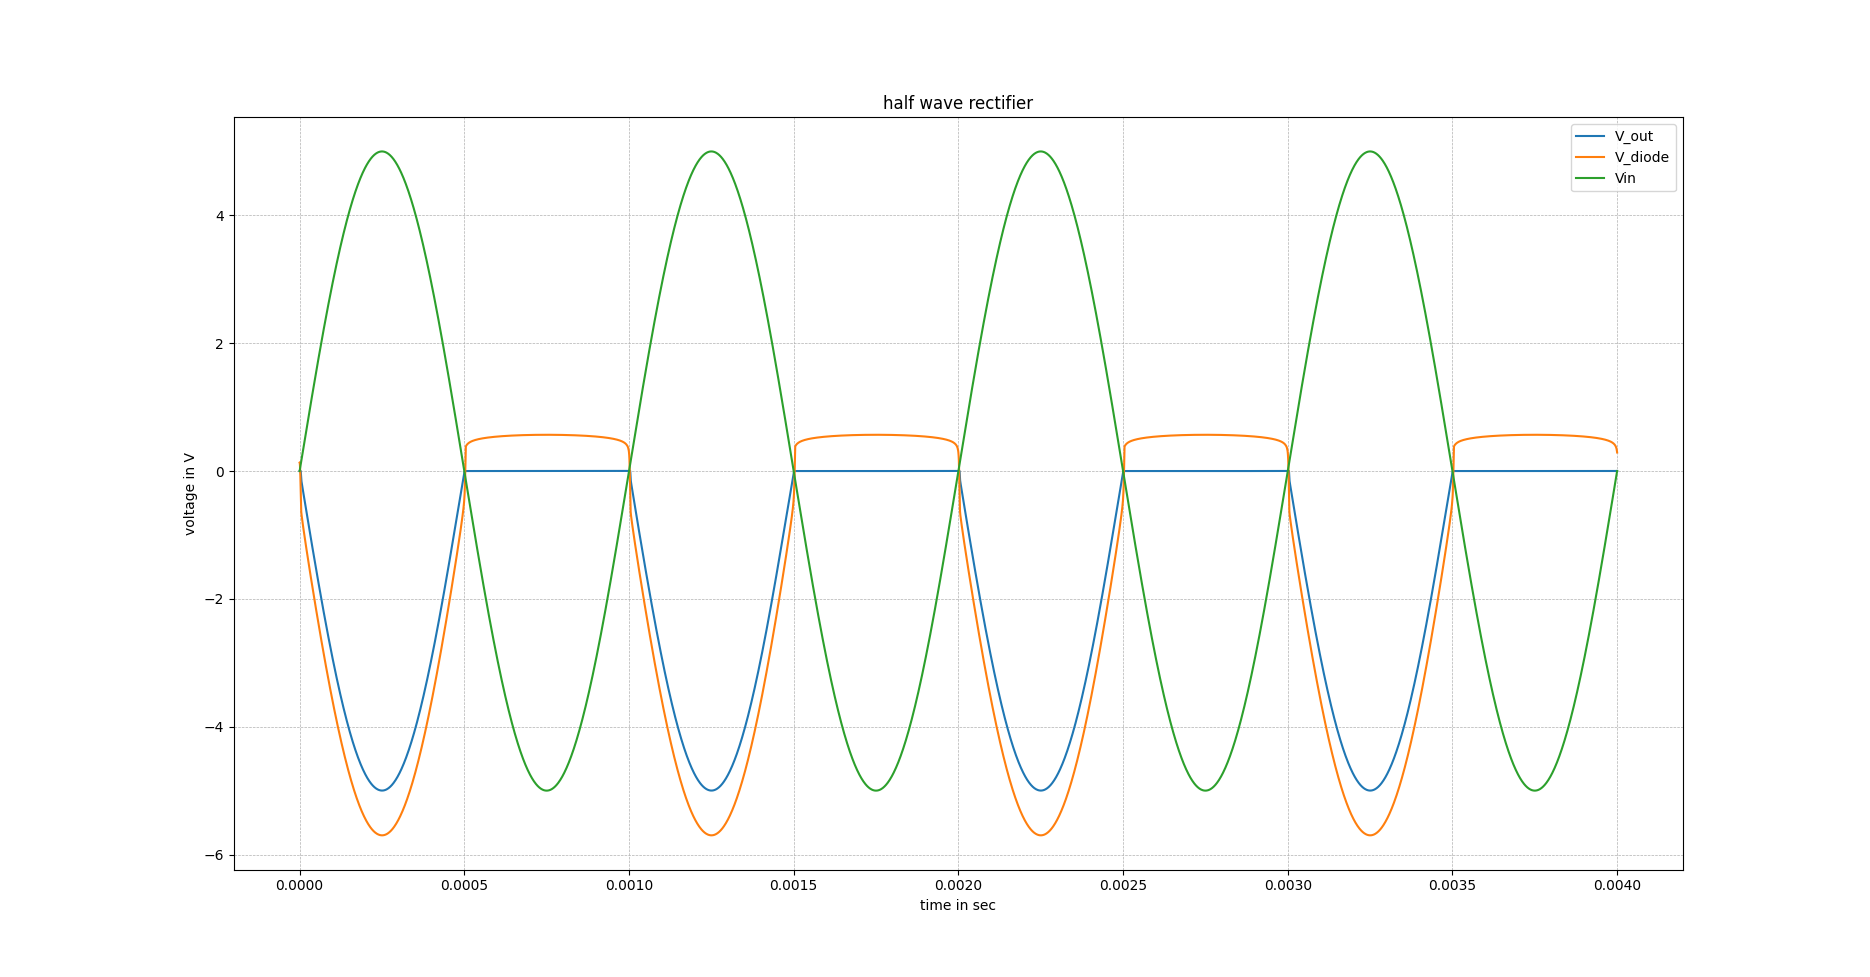
\includegraphics[scale = 0.4]{improved_half_wave_rectifier_plot.png}
\end{figure}
\newpage

\subsubsection{ full wave rectifier}
X-axis is time axis, Y-axis is voltage axis time vs \(V_{in}\), \(V_{out}\),\(V_{diode}\) is plotted below.  plot shows that when \(V_{in}\) is sinusodial , at \(V_{out}\) for both positive and negative part of sinusodial curve \(V_{out}\) remains positive , \(V_{out}=|V_{in}|\)
\begin{figure}[h!]
\centering
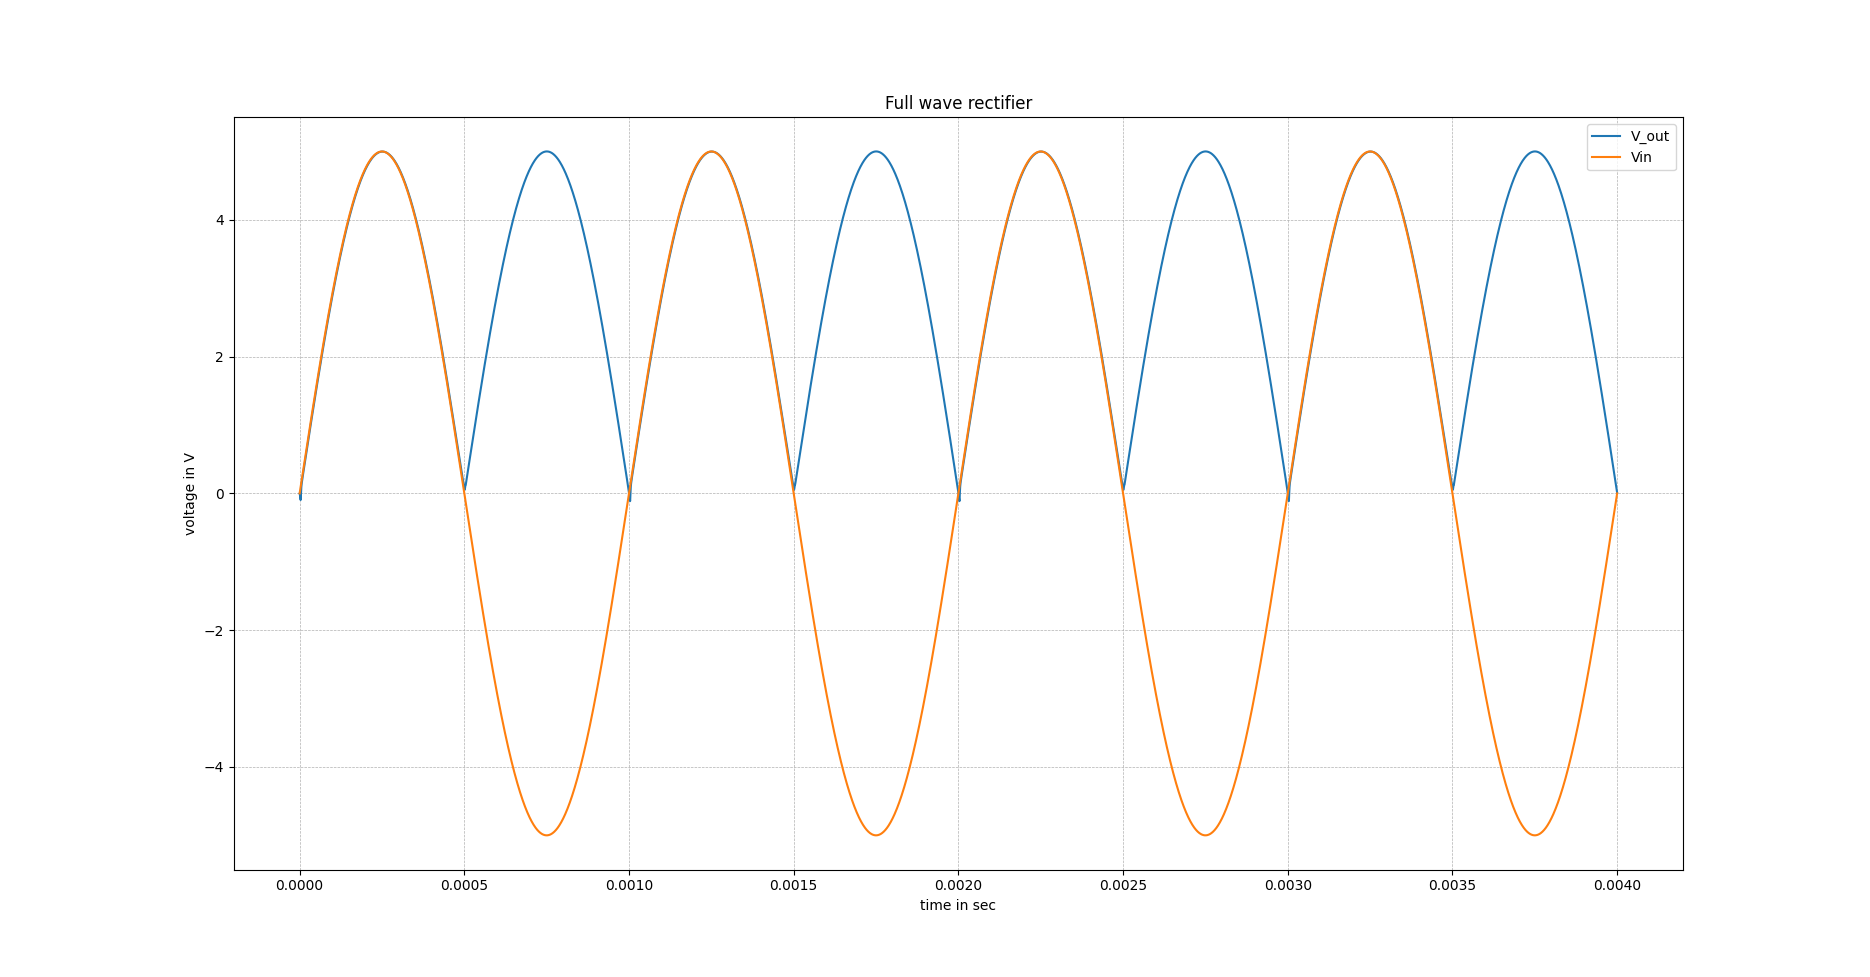
\includegraphics[scale = 0.4]{full_wave_rectifier_plot.png}
\end{figure}
\newpage

\section{Experiment completion status}
I have completed all sections in Lab only.

\end{document}
